\chapter{Introducción}
\label{sec:intro}

La aplicación de aprendizaje no supervisado para la agrupación (Clustering) de nodos en una red es un problema que ha sido estudiado ampliamente, la agrupación de redes completas por otro lado, es un problema que no se ha explorado ampliamente debido a la complejidad de hacer una comparación entre distintas redes. Recientemente el concepto de roles de nodos ha sido propuesto junto a sus características topológicas para estudiar distintas redes. En este trabajo se propone una metodología para realizar un agrupamiento de redes temáticas de Twitter utilizando aprendizaje no supervisado mediante una caracterización de las redes utilizando Órbitas para identificar roles estructurales de los usuarios dentro de la red.

\paragraph{Tipografía e tamaño de fonte:} Débese usar un único tipo de letra para cada un dos elementos que compoñen a memoria (é dicir, unha vez seleccionado o tipo de letra para o texto principal non se debe modificar, o mesmo para os subtítulos, táboas, notas ao pé de páxina, bibliografía, números de páxina, etc.). O tamaño de letra recomendado é de 11 puntos. 



%\verb|\marginparwidth|: \printinunitsof{cm}\prntlen{\marginparwidth}
\begin{figure}[htbp!]
    \centering
     %\pagediagram
    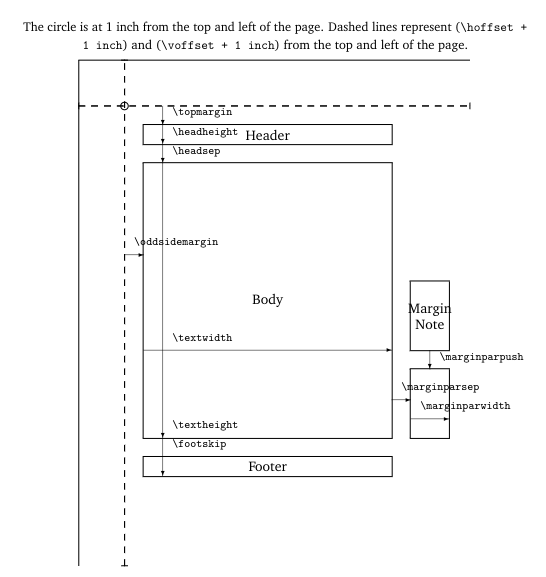
\includegraphics[width=\textwidth]{graphlet-thesis/images/layout.png}
    \caption{Dimensións das marxes utilizadas neste documento}
    \label{fig:layout}
\end{figure}

\paragraph{Tamaño do papel e marxes:} Utilizaráse un tamaño de papel A4, cos valores recomendadas para as marxes mostrados a continuación (véxase a figura \ref{fig:layout}).

\begin{center}
\begin{tabular}{ l l }
\textbackslash paperheight= 845.04694pt & \textbackslash paperwidth= 597.50793pt \\ 
\textbackslash hoffset= 0.0pt & \textbackslash voffset= 0.0pt \\
\textbackslash evensidemargin= 15.45935pt & \textbackslash oddsidemargin= 42.72656pt \\
\textbackslash topmargin= -39.24942pt & \textbackslash headheight= 17.0pt \\
\textbackslash headsep= 20.40001pt & \textbackslash textheight= 636.60028pt \\
\textbackslash textwidth= 394.78204pt & \textbackslash footskip= 185.0pt \\
\textbackslash marginparsep= 12.8401pt & \textbackslash marginparpush= 6.11995pt \\
\textbackslash columnsep= 10.0pt & \textbackslash columnseprule= 0.0pt \\
1em = 10.95pt  & 1ex = 5.2779pt \\
\end{tabular}
\end{center}
%\printinunitsof{cm}{\pagevalues}


\paragraph{Numeración das páxinas:} Tódalas páxinas deben estar numeradas, agás as que non teñan ningún contido ou a páxina de título. As páxinas non numeradas contan ingualmente. Por exemplo, a páxina de título é a  páxina (i).

As páxinas iniciais (o resumo, as dedicacións, a táboa de contidos, etc.) están numeradas con números romanos.  A partir da primeira páxina do primeiro capítulo reiníciase a numeración con números arábigos e continúa consecutivamente ata o final da tese, incluíndo os apéndices.

\paragraph{Espazo entre liñas:} Úsase interliñado simple.  Os parágrafos sepáranse por unha liña en branco (non se sangra a primeira liña do mesmo). 

\paragraph{Títulos e numeración de figuras e táboas:}  Cada táboa, figura, ilustación etc. debe ter un título indicando o elemento que pretende representar ou ilustrar.  As táboas numéranse consecutivamente ao longo do documento. As figuras, ilustracións, etc. tamén se contan consecutivamente ao longo do documento.

\paragraph{Encabezamentos e subtítulos:}     Os títulos indican a organización do documento.     Os capíutulos, secccións e subseccións débense empregar ao longo do documento, sendo coherentes no estilo e posición de cada elemento.  Cada capítulo debe comezar nunha páxina impar. 

\paragraph{Citas bibliográficas:} Débese utilizar un estilo recoñecido (tal como IEEE, APA, etc.). Recoméndase encarecidamente o uso de unha ferramenta como BibLaTeX. 


\section{Organización en seccións}
\label{sec:organización}

Este documento mostra un exemplo da posible organización dunha memoria do TFM. Descríbense a continuación as distintas seccións. 

Non existe un número de páxinas mínimo ou máximo. Non obstante, a extensión dun TFM está habitualmente entre 40 e 80 páxinas. A lonxitude variará segundo o tema elixido e o método de análise, polo que a extensión final deberá ser decidido polo autor e os seus titores. 

Unha posible organización do TFM é a seguinte (as extensións son meramente orientativas): 

\begin{enumerate}[noitemsep]
    \item Páxina de Título (obrigatorio -- 1 páxina).
    \item Resumo en inglés (\textit{abstract} -- obrigatorio -- 1 páxina).
    \item Resumo en galego ou castelán (obrigatorio -- 1 páxina).
    \item Agradecementos (opcional).
    \item Táboa de contidos (obrigatorio).
    \item Introdución (3-10 páxinas).
    \begin{enumerate}[noitemsep]
        \item Motivación.
        \item Obxectivos e presentación do problema que se vai resolver.
        \item Estrutura do documento.
    \end{enumerate}
    \item Situación actual (arpoximadamente 10-20 páxinas). Repaso do traballo relacionado, das tecnoloxías básicas, do punto de partida, etc. 
    \begin{enumerate}[noitemsep]
        \item Traballo relacionado.
        \item Tecnoloxías base.
        \item Marco de traballo (marco teórico, tecnolóxico, etc.).
    \end{enumerate}
    \item Descrición do traballo realizado (aproximadamente 10-20 páxinas). 
    \begin{enumerate}[noitemsep]
        \item Datos analizados.
        \item Análise teórica.
        \item Deseño (arquitectura, ataque, etc.).
        \item Descrición dos métodos. 
        \item Desenvolvementos realizados.
        \item Mecanismos para garantir a calidade do traballo.
    \end{enumerate}
    \item Resultados (aproximadamente 5-20 páxinas)
    \begin{enumerate}[noitemsep]
        \item Descrición dos resultados.
        \item Análise e discusión dos resultados / Validación.
    \end{enumerate}
    \item Conclusións (aproximadamente 5-10 páxinas).
    \begin{enumerate}[noitemsep]
        \item Resumo do traballo.
        \item Implicacións dos resultados / Impacto ecnonómico-social..
        \item Limitacións do traballo.
        \item Traballo futuro.
    \end{enumerate}
    \item Bibliografía (obrigatorio).
    \item Apéndices (opcional).
    \begin{enumerate}[noitemsep]
        \item Descrición de ferramentas.
        \item Descrición de configuración.
        \item Código. 
        \item Detalle adicional para algunha sección. 
        \item Etc. 
    \end{enumerate}
\end{enumerate}



\section{Obxectivos e presentación do problema}
\label{sec:intro:motivación}
{
\color{gray}
\Blindtext[3][1]

\cite{Jurgens:2000,Jurgens:1995,Miede:2011,Kohm:2011,Apple:keynote:2010,Apple:numbers:2010,Apple:pages:2010}

\cite{WEB:GNU:GPL:2010,WEB:Miede:2011}
}

\subsection{Metodoloxía}
\label{sec:intro:results:refs:method}
{
\color{gray}
\Blindtext[1][2]
}

\paragraph{Estratexia 1}
{
\color{gray}
\Blindtext[1][1]
}

\begin{lstlisting}[language=Python, caption={This simple helloworld.py file prints Hello World.}\label{lst:pyhelloworld}]
#!/usr/bin/env python
print "Hello World"
\end{lstlisting}

\paragraph{Estratexia 2}
{
\color{gray}
\Blindtext[1][1]
}

\begin{lstlisting}[language=Python, caption={This is a bubble sort function.}\label{lst:pybubblesort}]
#!/usr/bin/env python
def bubble_sort(list):
    for num in range(len(list)-1,0,-1):
        for i in range(num):
            if list[i]>list[i+1]:
                tmp = list[i]
                list[i] = list[i+1]
                list[i+1] = tmp

alist = [34,67,2,4,65,16,17,95,20,31]
bubble_sort(list)
print(list)
\end{lstlisting}

\section{Organización da memoria}
\label{sec:intro:organización}

\textbf{Capítulo \ref{sec:related}} \\[0.2em]
{
\color{gray}
\blindtext
}

\textbf{Capítulo \ref{sec:system}} \\[0.2em]
{
\color{gray}
\blindtext
}


\textbf{Capítulo \ref{sec:results}} \\[0.2em]
{
\color{gray}
\blindtext
}

\textbf{Capítulo \ref{sec:results}} \\[0.2em]
{
\color{gray}
\blindtext
}

\textbf{Capítulo \ref{sec:conclusion}} \\[0.2em]
{
\color{gray}
\blindtext
}